\chapter{Threshold Approach Results\label{app:a}}

\section{HMMs with states 2,3,4 testing for 1st group of data}
\begin{table}
\centering
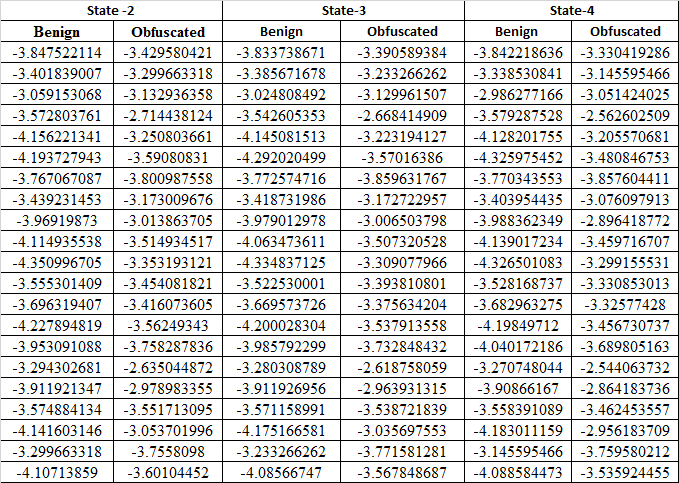
\includegraphics[width=1.0\textwidth]{images/a_1.png}
\caption{Table for first group of data} 
\label{table:Table for first group of data}
\end{table}
\pagebreak

\section{HMMs with states 2,3,4 testing for 2nd group of data}
\begin{table}
\centering
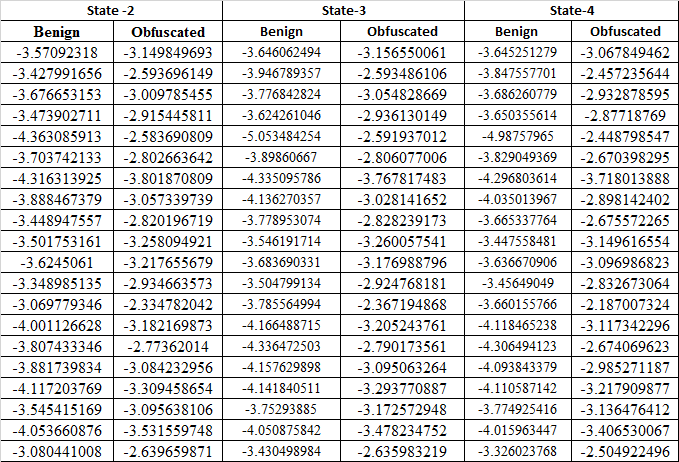
\includegraphics[width=1.0\textwidth]{images/a_2.png}
\caption{Table for second group of data} 
\label{table:Table for second group of data}
\end{table}
\pagebreak

\section{HMMs with states 2,3,4 testing for 3rd group of data}
\begin{table}
\centering
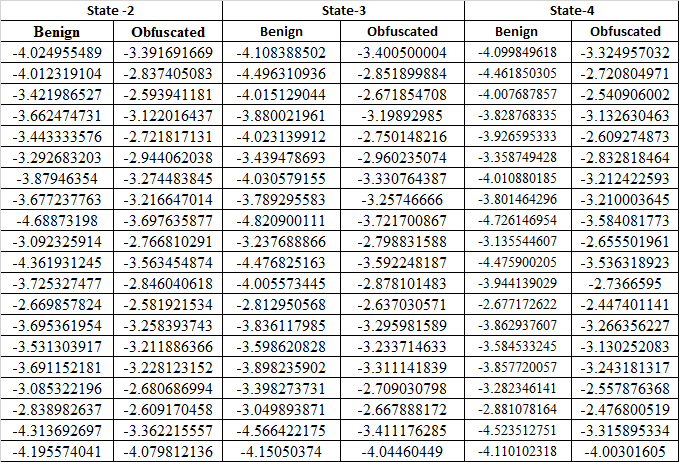
\includegraphics[width=1.0\textwidth]{images/a3.png}
\caption{Table for third group of data} 
\label{table:Table for third group of data}
\end{table}
\pagebreak

\section{HMMs with states 2,3,4 testing for 4th group of data}
\begin{table}
\centering
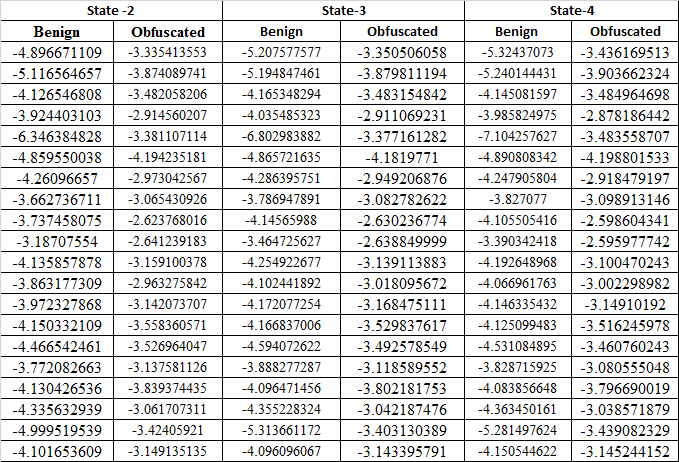
\includegraphics[width=1.0\textwidth]{images/a4.png}
\caption{Table for fourth group of data} 
\label{table:Table for fourth group of data}
\end{table}
\pagebreak

\section{HMMs with states 2,3,4 testing for 5th group of data}
\begin{table}
\centering
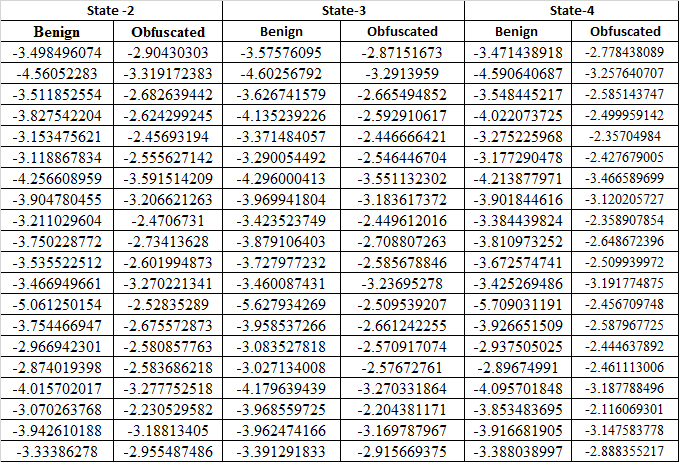
\includegraphics[width=1.0\textwidth]{images/a5.png}
\caption{Table for fifth group of data} 
\label{table:Table for fifth group of data}
\end{table}
\pagebreak